\message{ !name(lab1.tex)}\documentclass[a4paper,12pt,openany]{book}
\usepackage[T1]{fontenc}
\usepackage{amsmath}
\usepackage[latin1]{inputenc}
\usepackage{titlesec}
\usepackage{booktabs}
\usepackage{graphicx}
\usepackage[table,xcdraw]{xcolor}
\usepackage{romannum}
\usepackage{fancyhdr}
\usepackage{etoolbox}
\usepackage{float}
\usepackage{graphicx}
\usepackage{indentfirst}
\usepackage{geometry}
\geometry{
 a4paper,
 total={170mm,257mm},
 left=20mm,
 top=20mm,
 }
\pagestyle{fancy}
\fancyhf{} 
\fancyhead[RE,RO]{\thepage}
\fancyfoot[RE,RO]{P20IC013}
\fancyfoot[LE,LO]{Darsh Gajjar}

\patchcmd{\chapter}{\if@openright\cleardoublepage\else\clearpage\fi}{}{}{}

\titleformat
{\chapter} % command
[display] % shape
{\bfseries\Large\itshape} % format
{Process Control LAB Manual } % label
{0.5ex} % sep
{
    \rule{\textwidth}{1pt}
    \vspace{-0.5ex}
    \centering
} % before-code
[
\vspace{-0.5ex}%
\rule{\textwidth}{0.3pt}
] % after-code
\titlespacing*{\chapter}{5pt}{-50pt}{10pt}

%\titleformat{\section}[wrap]
%{\normalfont\bfseries}
%{\thesection.}{0.5em}{}

%\titlespacing{\section}{12pc}{1.5ex plus .1ex minus .2ex}{1pc}

\titleformat{\section}{\normalfont\fontsize{12}{15}\bfseries}{\thesection}{1.5em}{}

\setlength{\parindent}{3em}
\setlength{\parskip}{0.5em}
\begin{document}

\message{ !name(lab1.tex) !offset(-3) }

\chapter{Experiment : 01}

\section{Title : Introduction to MATLAB/Simulink: Plot the step response of first order and second
order systems.}


\section{Apparatus :}
MATLAB/Simulink Software \par

\section{Theory :}
let us consider first order system of which has transfer function is given below
\begin{equation}
  G_1(s) = \frac{1}{1 + s}
\end{equation}
\par and second order system which transfer function is
\begin{equation}
 G_2(s) = \frac{10}{s(s+15)}
\end{equation}
\par
Now evaluate the closed loop transfer function of above systems in which step
response is given as input and negetive unity feedback is used. general closed
loop transfer function is defined as below
\[  \frac{C(s)}{R(s)} = \frac{G(s)}{1 + G(s)H(s)} \]
\par

where $G(s)$ is  feed forward gain and $H(s)$ is feedback gain, where $C(s)$
referred as controlled ouput variable and $R(s)$ as reference set point or input
variable \par

as per above equation, we get $Y_1(s)$ and $Y_2(s)$ as first order and
second order closed loop transfer function respectively \par
\begin{equation}
  Y_1(s) = \frac{1}{s+2}
\end{equation}
\begin{equation}
  Y_2(s) = \frac{10}{s^2+15s+10}
  \pagebreak
\end{equation}
\section{Observation :}
\begin{center}
  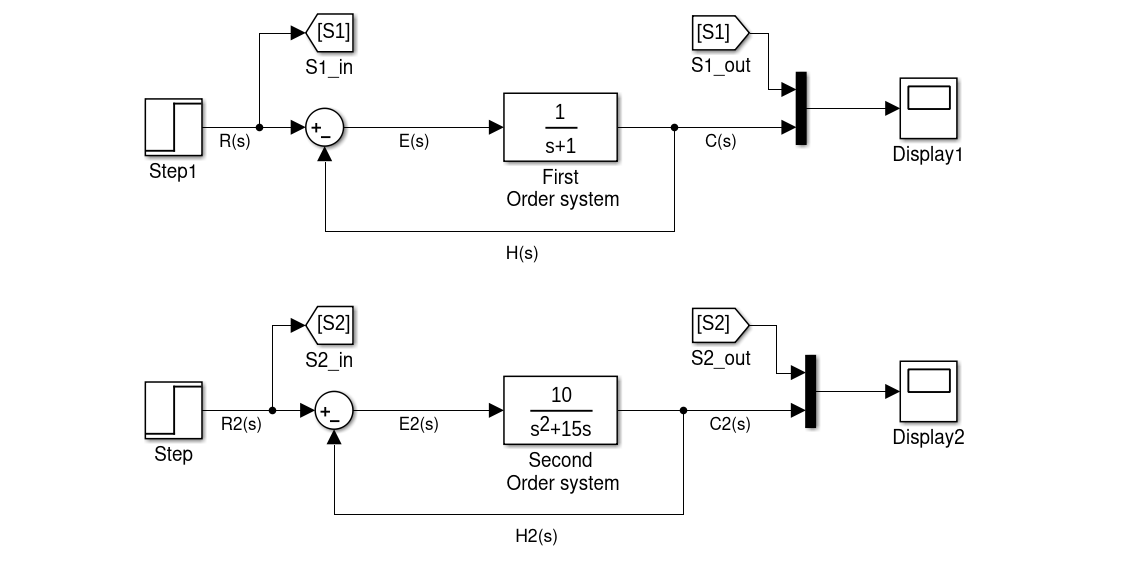
\includegraphics[width = 165mm, scale = 0.80]{lab1fig1.png}
  Figure 1.1 : Simulink model of system under consideration
\end{center}
\begin{figure}[h!]
  \begin{center}
  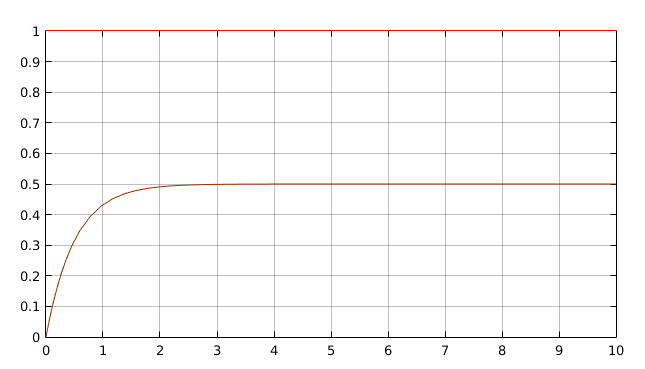
\includegraphics[width = 165mm, scale = 0.80]{graph1.png}
  Figure 1.2 : Step response of first order system
  \end{center}
\end{figure}
\begin{center}
  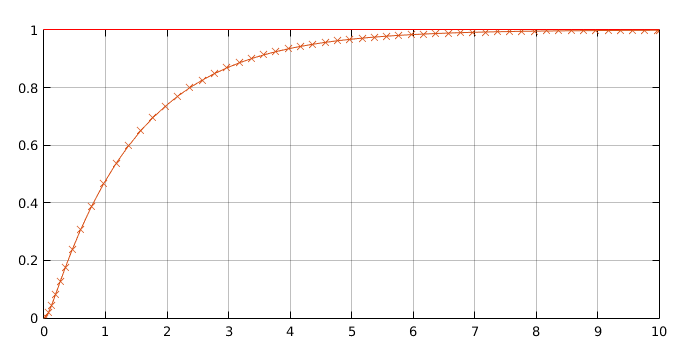
\includegraphics[width = 165mm, scale = 0.85]{graph2.png}
  Figure 1.3 : Step response of second order system
\end{center}
\section{Conclusion :}
\begin{itemize}
\item by giving step response or bounded input, we get an bounded output in both
  the systems, so they are behave as stable.
  \item first order system will settled down to final value at approx $~$2.2
    seconds when step input is given
    \item in second order system final value achieve at approx 7 seconds due to
      its Overdamped response.
\end{itemize}
\chapter{Experiment : 02}
\section{Title : Study the effect of varying system gain for a second order overdamped system, and
verifying the results using Root locus.}

\section{Aim :}
\begin{enumerate}
  \item {\bf Analyse the step responses of Second order system at different  values of $K_P$.}
\item {\bf Analyse the step response of Second order system with transportation delay with and
    without disturbances.}
 \end{enumerate} 
\section{Apparatus :}
MATLAB/Simulink Software \par
\section{Theory :}
In a first part we have $G_1(s)$ of second order system and varying the
proportional gain($K_P$) to 50, 100, 1500 values and evaluating its step
responses.
\begin{equation}
  G_1(s) = \frac{8}{s^2+50s}
\end{equation}
\par
In second part we have second order system with dead time or transportation
delay $G_2(s)$ and disturbance with delay as $G_3(s)$ defined below
\begin{eqnarray}
  G_2(s) = \frac{2e^{-5s}}{50s^2+15s+1} \\
  \\
  G_3(s) = \frac{0.3e^{-5s}}{15s+1}
\end{eqnarray}
\pagebreak
\section{Observation :}
\begin{figure}[ht!]
  \centering
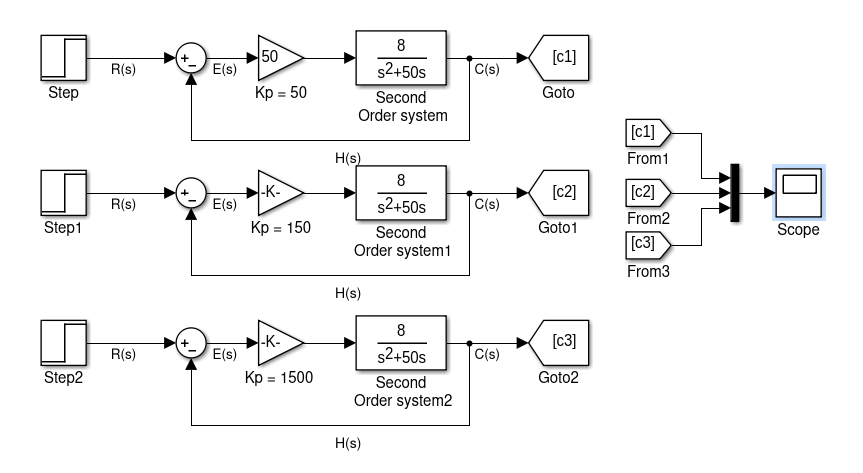
\includegraphics[width = 165mm, scale = 0.85]{lab2part11.png}
   \caption{Simulink model of above system}
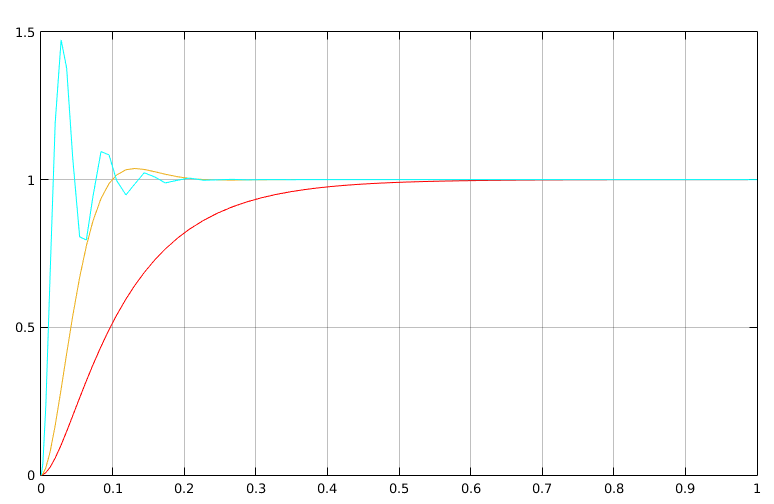
\includegraphics[width = 165mm, scale = 0.85]{lab2part12.png}
   \caption{Figure 2.2 : Step responses of second order system with different
     value of $K_p$}
 \end{figure}
\begin{minipage}{0.60\linewidth}
  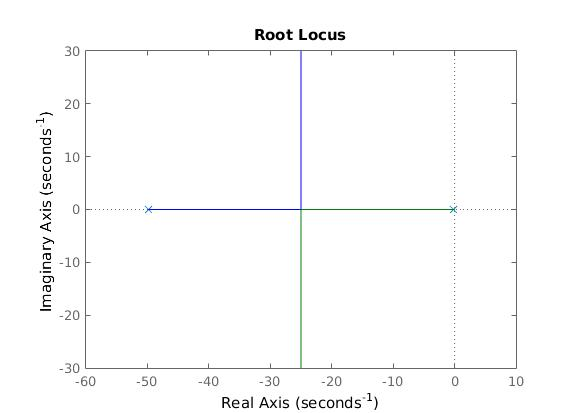
\includegraphics[width = \linewidth]{rlocus.jpg}
  \begin{center}
    \caption{Root locus of $G_1(s)$}
    \end{center}
    \end{minipage} \hfil
     \begin{minipage}{0.45\linewidth}
       \begin{verbatim}
#Code for plot Root locus
# in MATLAB  programme
num = [1];
den = [1 50 8];
G = tf(num,den);
rlocus(G)
\end{verbatim}
\end{minipage}
 \begin{figure}[ht!]
 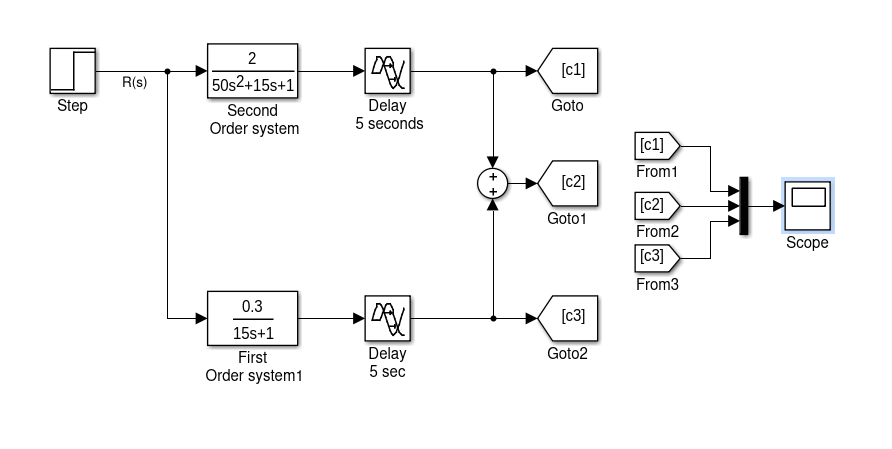
\includegraphics[width = 165mm, scale = 0.85]{lab2part21.png}
 \caption{Simulink Model of second order system with time delay}
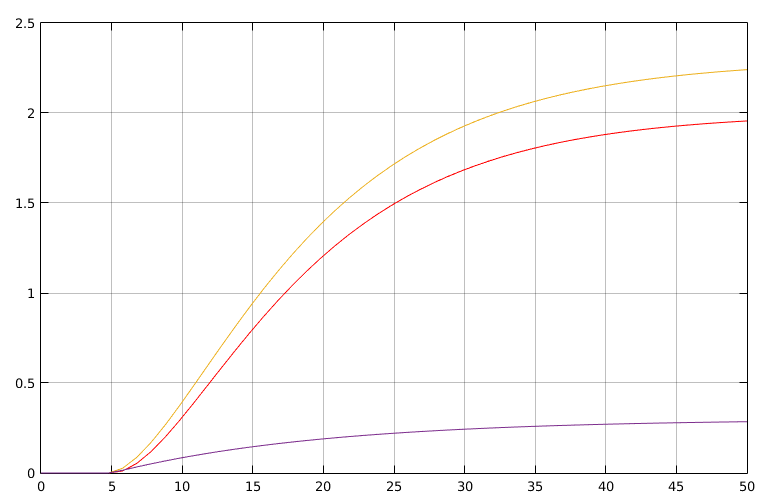
\includegraphics[width = 165mm, height = 63mm, scale = 0.95]{lab2part22.png}
\caption{Step responses of Second order system with dead time}
\end{figure}
\section{Conclusion :}
\begin{itemize}
\item In first part we have observed that on increasing the value of $K_P$ output response is reaching
at final value very fast. It is verified from Root locus that at $K_P$ = 50 we get critical damped
response while on  $K_P$ = 150, 1500 we get underdamped response i.e. having overshoot.
   \item In second part due to disturbance, output response is getting deviated from its
reference value and reaching at peak which is greater than input.
 \end{itemize}

\chapter{Experiment : 03}
\section{Title : Dynamic response of First order system with time delay}
\section{Aim :}
\begin{enumerate}
\item Plot the responses of firsr order system with given condition:
  \begin{enumerate}
  \item Exact response
  \item {\bf \Romannum{1} order Pad\'e} Approximation
  \item {\bf \Romannum{2} order Pad\'e} Approximation
  \end{enumerate}
\item Proportional only control of First order system with dead time
\item Intergral only control of Second order system with dead time
\end {enumerate}

\section{Apparatus :}
MATLAB/Simulink Software \par
\section{Theory :}
In a first part we have plant transfer function with transportation delay as $G_1(s)$
\begin{equation}
  G_1(s) = \frac{Ke^{-sT_d}}{sT_p + 1}
\end{equation}
\par
This is exact or actual transfer function, which we have to approximate using
Taylor series approximation by expanding transportation delay term into ints
factors into poles and zeros.Now First order Pad\'e approximation for a time delay
consist of half magnitude of right hand side s plane zero and half magnitude of
left hand side s plane pole, or ratio of two polynomials in 's' with with
coefficient term calculating by taylor series expansion of $e^{-s\theta}$.

\noindent First Order Pad\'e Approximation is,
\begin{center}
\scalebox{2.0}{$
  e^{-s\theta} = (\frac{1 - \frac{s\theta}{2}}{1 + \frac{s\theta}{2}})$}
\end{center}
second Order Pad\'e Aprroximation is,
\begin{center}
  \scalebox{2.0}{$
  e^{-s \theta} = \frac{1 - \frac{s \theta}{2} + \frac{s^2 (\theta)^2}{12} }{1 + \frac{s \theta}{2} + \frac{s^2 (\theta)^2}{12}}$}
\end{center}
\noindent For a first case we have $T_d$ = 5 second, $T_p$ = 10 second and K = 1, so we
have to evaluate the responses, so that
\begin{equation}
 G(s) = \frac{ e^{-5s}}{10s + 1}
\end{equation}
\Romannum{1} Order Pad\'e Approximation
\begin{equation}
  G_1(s) = \frac{1-2.5s}{25s^2+12.5s+1}
\end{equation} \\
\Romannum{2} Order Pad\'e Approximation
\begin{equation}
  G_2(s) = \frac{2.083s^2-2.5s+1}{20.83s^3+27.083s^2+12.5s+1}
\end{equation}
In second part firstly we analyse the response of G(s) at different values of
K=1.05, 1.15, 2, 4.5, 8.5 and selecting value of $T_d$ = 5 and $T_p$=1. \par
Now in second part we change value of $k_i$= 0.2,0.5,0.8,1 respectively and add
disturbance in system with time delay of 25 seconds.
\section{Observation :}
\begin{figure}[H]
  \centering
  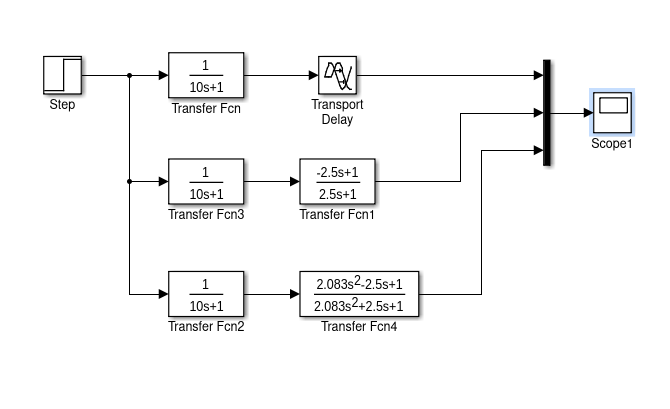
\includegraphics[width = 165mm, scale = 0.85]{lab03part1.png}
  \caption{Simulink model of system of part 1}
\end{figure}
\pagebreak
\begin{figure}[H]
  \centering
  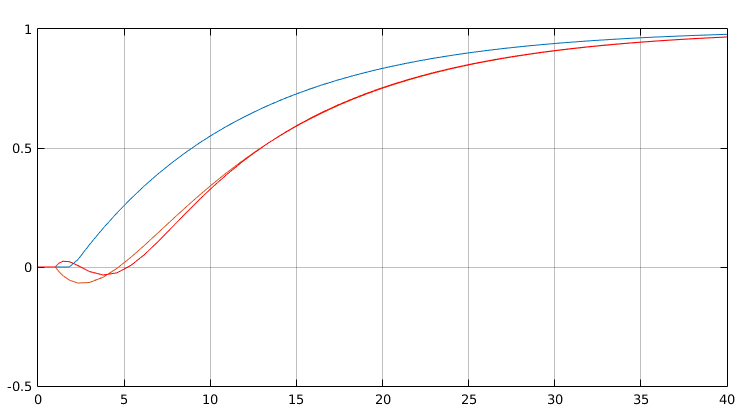
\includegraphics[width = 165mm, scale = 0.85]{lab03part12.png}
  \caption{step response of All system in combined axis}
   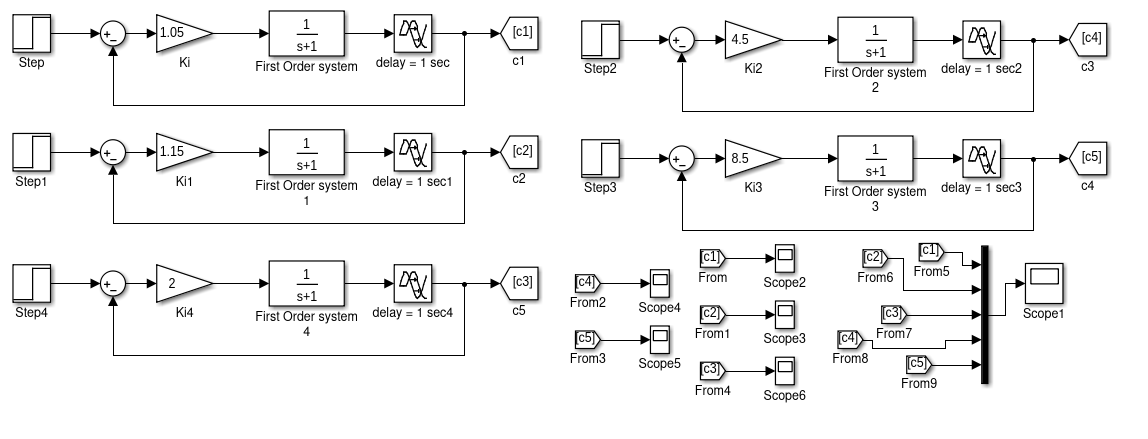
\includegraphics[width = 165mm, height = 80mm, scale = 0.85]{lab03part2a.png}
   \caption{simulink model of part 2}
   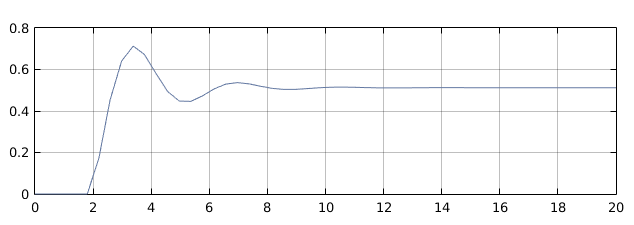
\includegraphics[width = 165mm, scale = 0.85]{lab03part2a1.png}
   \caption{step response with $K$ = 1.05}
 \end{figure}
 \begin{figure}[H]
   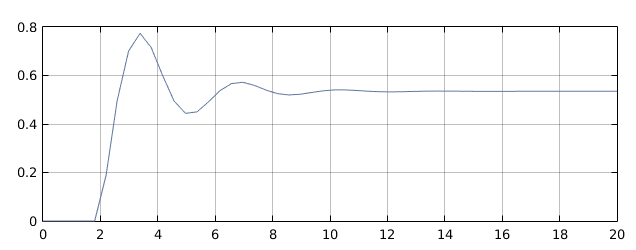
\includegraphics[width = 165mm, scale = 0.85]{lab03part2a2.png}
   \caption{step response with $K$ = 1.15}
   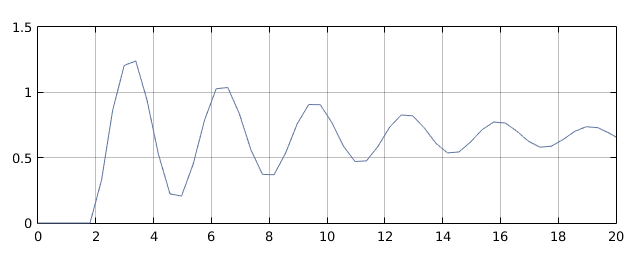
\includegraphics[width = 165mm, scale = 0.85]{lab03part2a3.png}
   \caption{step response with $K$ = 2}
   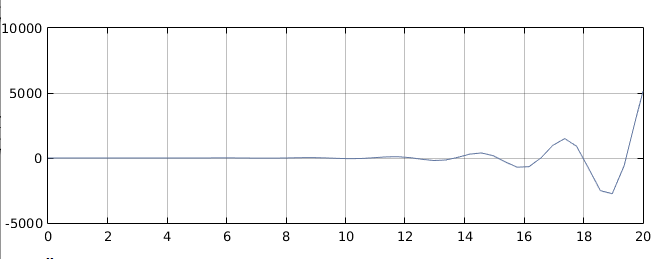
\includegraphics[width = 165mm, scale = 0.85]{lab03part2a4.png}
   \caption{step response with $K$ = 4.5}
 \end{figure}
 \begin{figure}[H]
  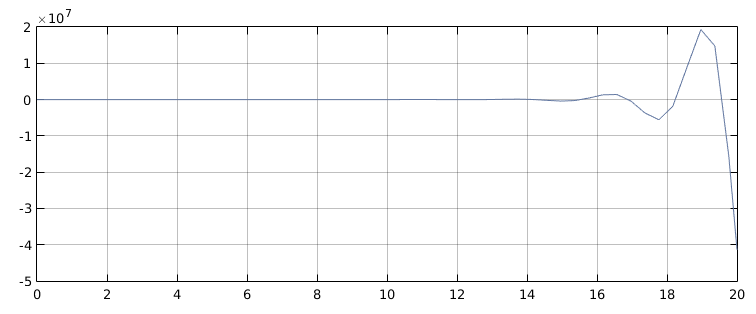
\includegraphics[width = 165mm, scale = 0.85]{lab03part2a5.png}
  \caption{step response with $K$ = 8.5}\\
  \vfil
 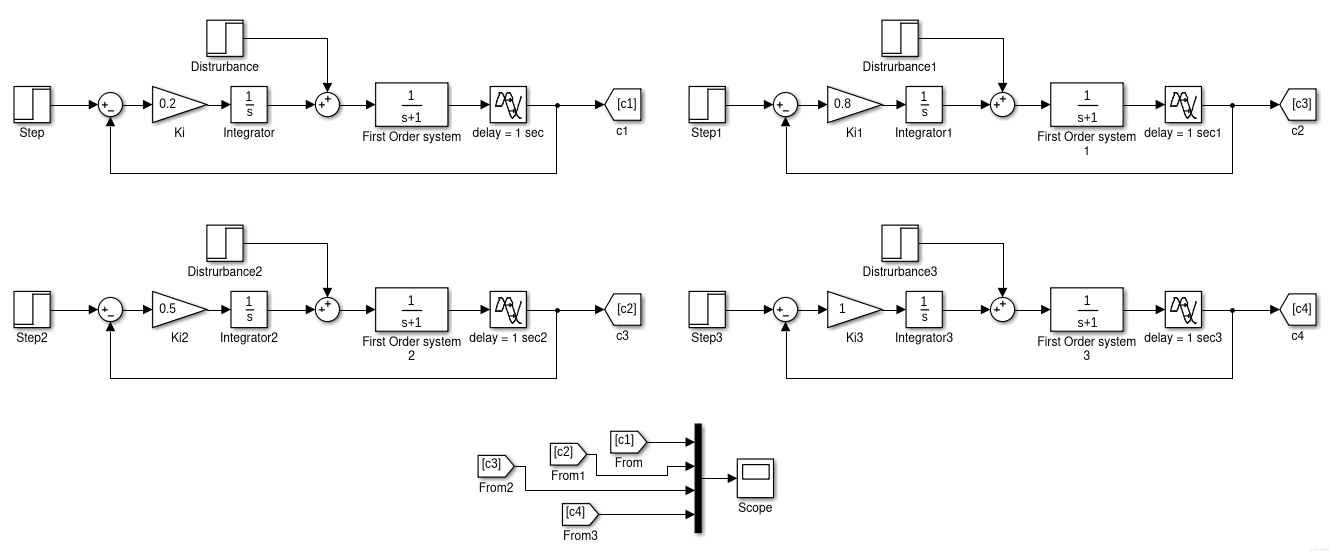
\includegraphics[width = 165mm, height = 110mm, scale = 0.85]{lab03part21.png}
 \caption{simulink model of system of part 3}
\end{figure}
\begin{figure}[H]
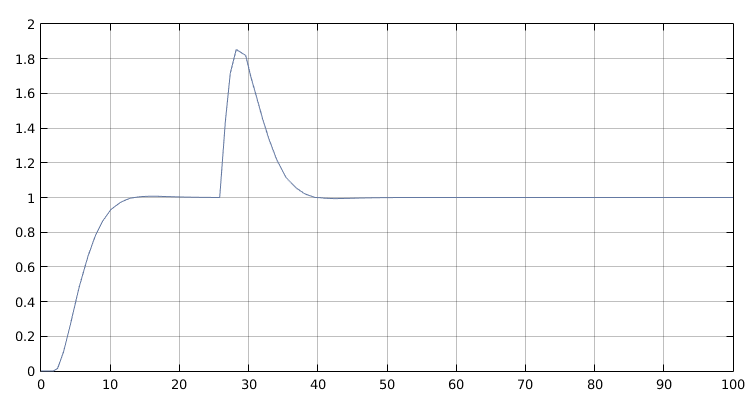
\includegraphics[width = 165mm, height=55mm, scale = 0.85]{lab03part22_ki_0_2.png}
 \caption{step response with $K_i= 0.2$}
 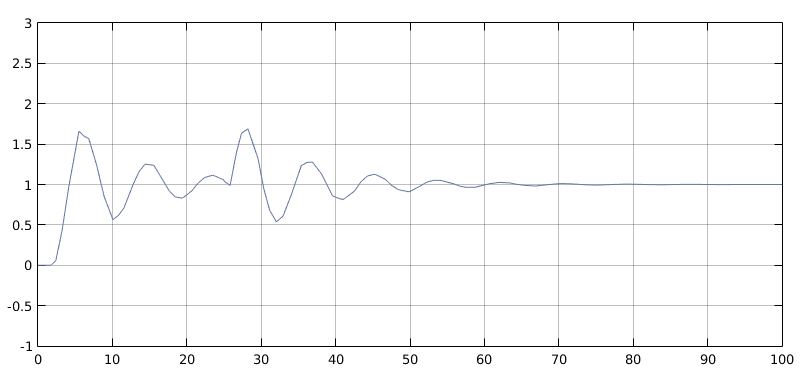
\includegraphics[width = 165mm, height =55mm, scale = 0.85]{lab03part23_k_i_0_5.png}
 \caption{step response with $K_i= 0.5$}
 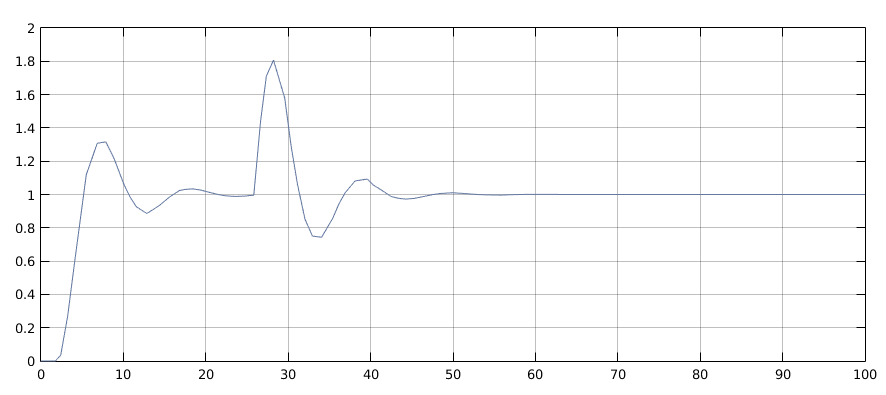
\includegraphics[width = 165mm, height=55mm, scale = 0.85]{lab03part24_k_i_0_8.png}
 \caption{step response with $K_i= 0.8$}
 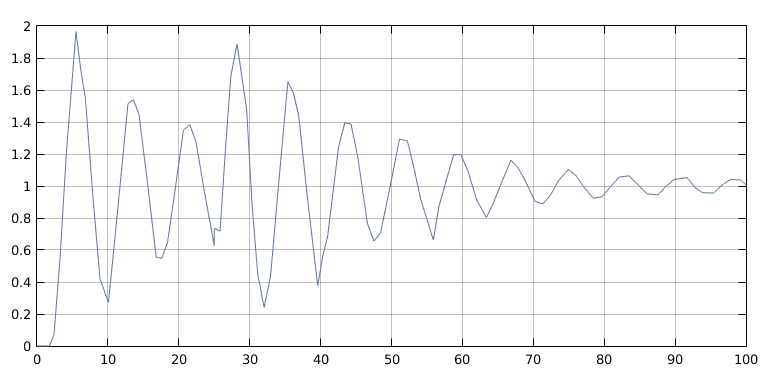
\includegraphics[width = 165mm, height=55mm, scale = 0.85]{lab03part25_k_i_1.png}
 \caption{step response with $K_i= 1$}
\end{figure}
\section {Conclusion}
\begin{itemize}
\item In First Part of system we can verify that system incorporate inverse
    response when pad\'e approximation is used, in which initial slope is
    negetive and response goes to reverse direction to the reference value.
\item  Also if we increase order of pad\'e approximation then inverse
     response increase or become double.
\item In second part as value of K (gain) is increased then its step response has
       increasing time delay and oscillation respectively.
\item Now in Third part, for analysis of integral control only we had
         inserted additional disturbance of step input after 25 sec and check
         that system will become oscillatory in first some cycle of operation as
         value of $K_i$ is increasing.
\end{itemize}

\chapter{Experiment : 04}
\section{Title : Approximation of Higher order system into first and second order systems with time
delay using Taylor series approximation and Skogestad's Half rule.}
\section{Apparatus :}
MATLAB Software
\section{Theory :}
For Approximation of system, we need to linearized higher order nonlinear model
into its equivalent first order or second order model so we can deal easily with
its dynamic and steady and state characteristics. So that we are using methods
like Taylor series and SKOGESTAD's Half rule. \par 
\noident Tailor series approximation is expressed up to second term,so that
\begin{eqnarray}
  e^{-\theta s} \approx 1 - \theta s\\
   e^{-\theta s} = \frac{1}{e^{\theta s}} \approx \frac{1}{ 1 + \theta s}
\end{eqnarray}
Now from SKOGESTAD's methods, there are some rules to transform higher order
system into first order or second order equivalent system is given below
\begin{itemize}
\item if model has multiple time constants than manipulation takes place with
    largest neglected Time constant
\item in denominator one half of neglected T is added to the existing time
      delay and other half of neglected T is added to the time constant that is
      retained
\item Third largest time constants that are smaller than largest neglected
        T will be considered \& added as time delay term
\end{itemize}
\scalebox{1.25}{\bf Part : A}
\begin{equation}
  G(s) = \frac{K(-0.1s + 1)}{(5s+1)(3s+1)(0.5s+1)}
  \end{equation}
  \noindent Derive an approximation First order plus time delay model(FOPTD) using:
  \begin{itemize}
  \item Taylor series approximation
  \item SKOGESTAD's Half rule
  \end{itemize}
  we get our transform or linearized plant transfer function as
  \begin{equation}
  G_{T}= \frac{Ke^{-3.6s}}{5s + 1},  G_H = \frac{Ke^{-2.1s}}{6.5s + 1}  
  \end{equation}
  where $G_T$ = approximated transfer function using taylor series\\
  $G_H$ =  approximated transfer function using SKOGESTAD's half rule\\
  \par
 \noindent \scalebox{1.25}{\bf Part : B}
 \begin{equation}
   H(s) = \frac{K(1 - s)e^{-s}}{(12s+1)(3s+1)(0.2s+1)(0.05s+1)}
 \end{equation}
   \noindent Derive models using Skogestad's rule:
   \begin{itemize}
   \item First order plus time delay
   \item Second order plus time delay take K = 1
 \end{itemize}
   \par
   we get transformed approximated plant transfer function as
\begin{equation}
   H_{T1}(s)= \frac{e^{-3.75s}}{13.5s + 1},  H_{H2}(s) = \frac{Ke^{-2.15s}}{(12s + 1)(3.1s + 1)}
 \end{equation}
 \section{Observation : }
 \begin{subfigure}
\begin{center}
  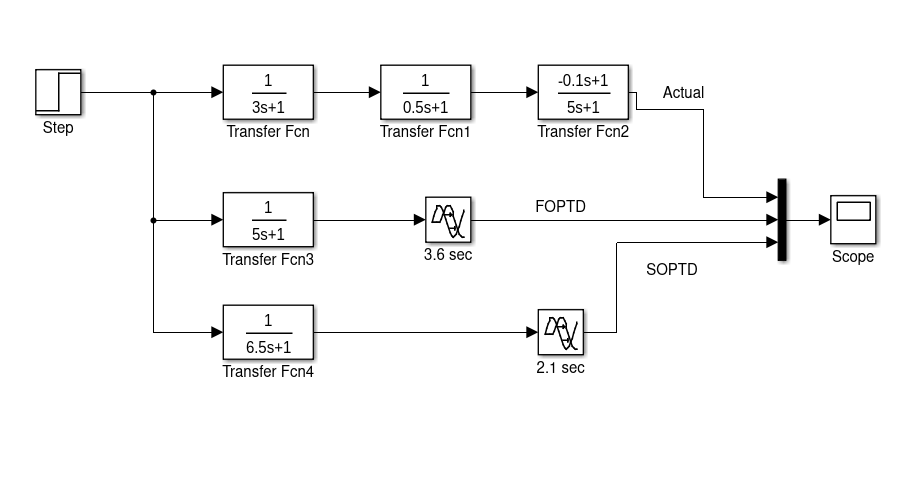
\includegraphics[width=165mm, scale=0.95]{lab04part10.png}
  \caption{Simulink model of systems given is Part A}
\end{center}
\end{subfigure}
  \begin{figure}[H]
    \centering
    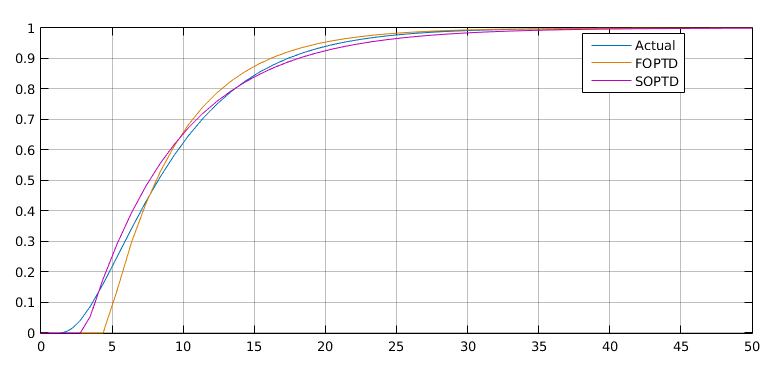
\includegraphics[width=165mm, scale=0.95]{lab04part11.png}
    \caption{Step response of system with time delay}
   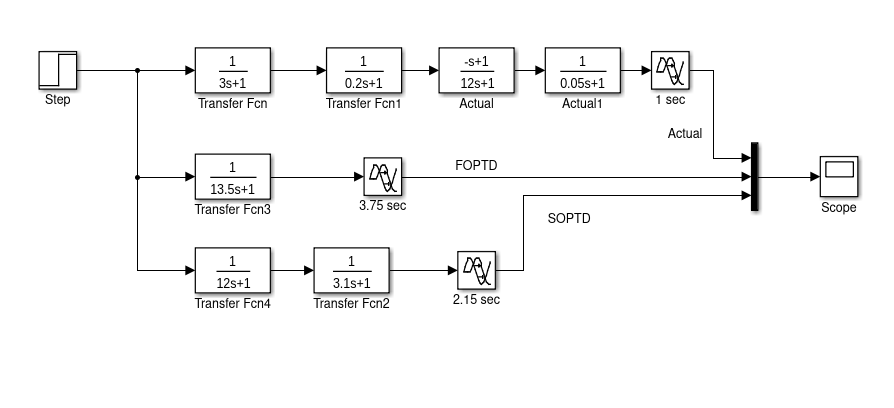
\includegraphics[width=165mm,scale=0.85]{lab04part20.png}
   \caption{Simulink model of systems given in Part B}
  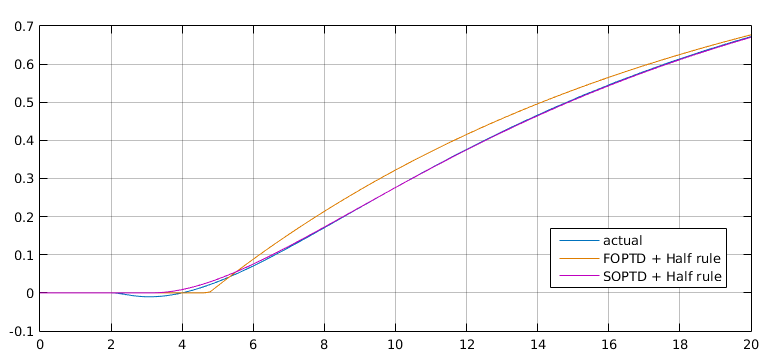
\includegraphics[width=165mm,scale=0.85]{lab04part21.png}
  \caption{Step response of system approximated by Half rule}
  \end{figure}
\section{Conclusion : }
\begin{itemize}
  \item In part A we get the more time delay in Half rule approximation, then in Taylor series
approximation in output response but settling time is almost same.
\item In part B we get little spike in actual response. But in approximation we do not get any
spike. Here FOPTD has more delay than SOPTD, and no changes in other characteristics.
\end{itemize}
\chapter{Experiment : 05}
\section{Title : Study of offset in a response of First order system with proportional controller, and
eliminating it using PI controller.}

\section{Apparatus :}
MATLAB/Simulink software

\section{Theory :}
there is a plant $G_p(s)$ has first order transfer function and controller
transfer function is
termed as $G_c(s)$, we are giving step response to the closed loop unity
feedback system in which,

\begin{equation}
  G_p(s) = \frac{K_p}{1 + s\tau_p},    G_c(s) = K_c(\frac{1+ s\tau_i}{s\tau_i})  
 \end{equation}\\
 \scalebox{1.25}{\bf Part A}
  \\
  first we apply proportional controller, i.e. $K_c$ to first order system and
  analyse offset which is difference between actual value and desired value of
  response.
  Now Closed loop transfer function in this case is,
 \begin{equation}
    H_{cl}(s)=\frac{C(s)}{R(s)} = \frac{K_c K_p}{1 + K_cK_p+ s T_p}
 \end{equation}
    here $K_p$ = 1, $T_p$ = 5,
    Applying Routh's stability criterion, we get stability condition as
\begin{align}
      T_p &> 0 \\
     (1 + K_pK_c) &> 0\\
     K_p K_c &> -1
\end{align}
here we need to change the value of $K_c$ = -2,-0.5,1,5,10 and analyse the
response of c(t), u(t),and its offset.

\noindent\scalebox{1.25}{\bf Part B}\par
\noindent In this part we are using PI controller to cotrol the behavious of plant tansfer
function and eliminate offset of proportional controller, so that closed
transfer function of entire system is

\begin{equation}
  Y_{cl}(s) = \frac{G_c(s)G_p(s)}{1 + {G_c(s)G_p(s)}}
\end{equation}\pagebreak
\\
  After substituting values
\begin{center}
  \scalebox{2.0}{$
    Y_{CL} = \frac{1 +s \tau_i}{\frac{\tau_p \tau_i}{K_c K_p}s^2 +\frac{\tau_i(1 + K_pK_c)}{K_pK_c}s + 1}
    $}
  \end{center}
  Now applying Routh Hurwitz's stability criteria to $Y_{CL}$ and $\tau_i \tau_p
  > 0$ so that
 \begin{align*}
    \frac{\tau_i \tau_p}{K_cK_p} &> 0 \\
    \frac{\tau_i(1+K_pK_c)}{K_cK_p} &> 0 \\
    K_p K_c &> 0    
 \end{align*}

here $\tau_p$ = 5, $K_i$ = 0.2, 4,($\tau_i$ = 0.25,5) and $K_c$ = 5 and obeserve that whether offset is
eliminated by PI only control or not.
\section{Observation :}
\begin{figure}[h!]
  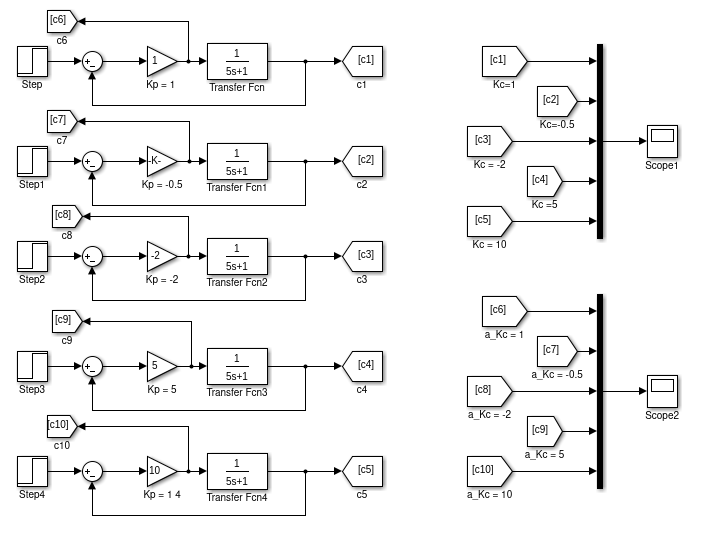
\includegraphics[width = 165mm, scale = 0.85]{lab05part01.png}
  \caption{Simulink model of system for proportional control only}
\end{figure}
\begin{figure}[H]
  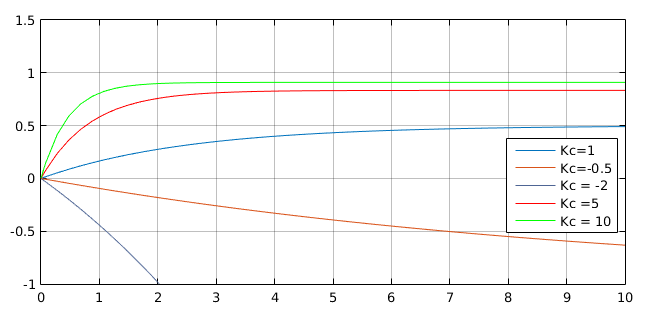
\includegraphics[width = 165mm, scale = 0.85]{lab05part11.png}
  \caption{step response of systems with different value of $K_c$}
  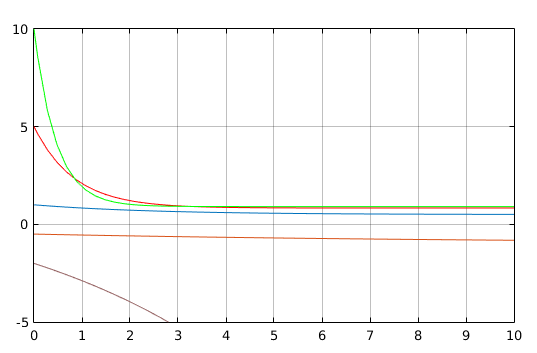
\includegraphics[width = 165mm, scale = 0.85]{lab05part12.png}
  \caption{controller response of systems with different value of $K_c$} 
\end{figure}
 \begin{figure}[H]
   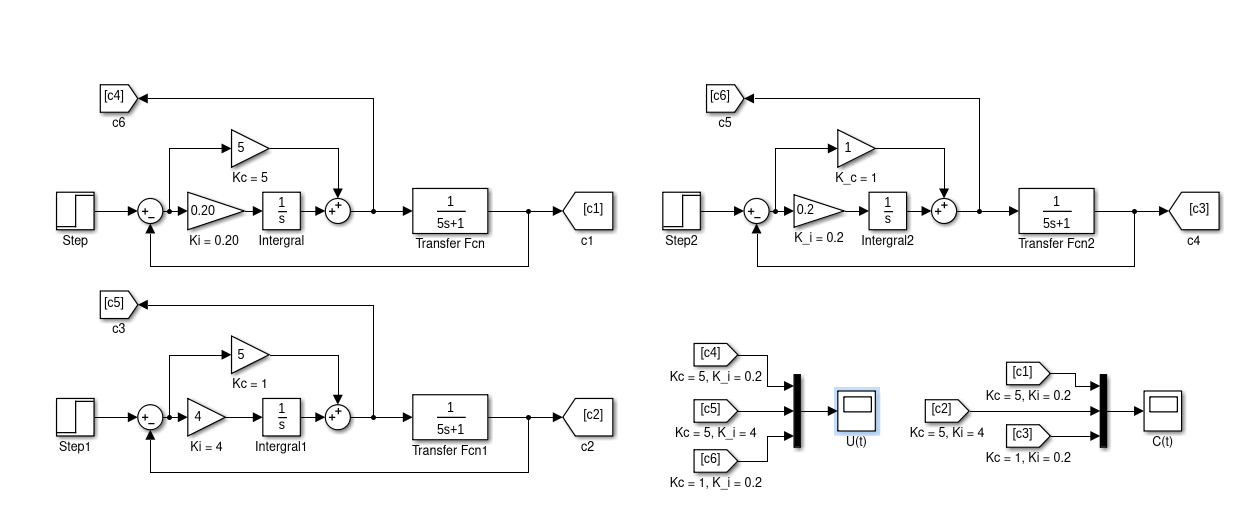
\includegraphics[width = 165mm, height = 100mm, scale = 0.95]{lab05part20.png}
   \caption{simulink model of systems given in Part B}
   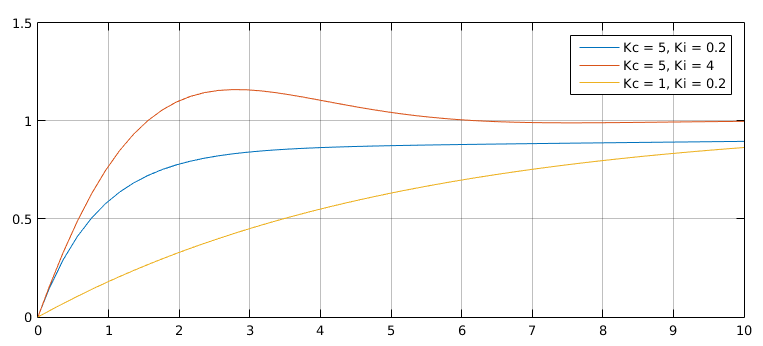
\includegraphics[width = 165mm,height = 65mm, scale = 0.85]{lab05part21.png}
   \caption{step response of systems with different value of $K_i$}
  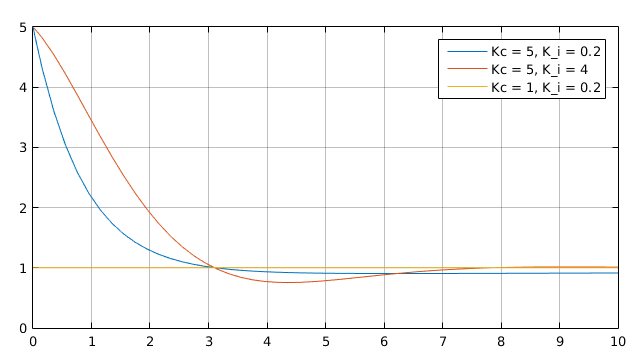
\includegraphics[width = 165mm, height = 65mm, scale = 0.85]{lab05part22.png}
  \caption{controller response of systems with different value of $K_i$}
 \end{figure}







  
\section{Result :}


\begin{table}[H]
\centering
\resizebox{\textwidth}{!}{%
\begin{tabular}{@{}llll@{}}
\toprule
\rowcolor[HTML]{F0BB65} 
Value of Kc &
  \begin{tabular}[c]{@{}l@{}}Nature of response\\ C(t)\end{tabular} &
  \begin{tabular}[c]{@{}l@{}}Offset\\ E(s) = 1/(1+KpKc)\end{tabular} &
  \begin{tabular}[c]{@{}l@{}}Condition\\ of Kc \& Kp\end{tabular} \\ \midrule
10 & \begin{tabular}[c]{@{}l@{}}Stable and \\ Overdamped\end{tabular} & 0.091 & \begin{tabular}[c]{@{}l@{}}Same sign\\ Kp Kc \textgreater 0\end{tabular}   \\
5  & \begin{tabular}[c]{@{}l@{}}Stable and\\ Overdamped\end{tabular}  & 0.168 & \begin{tabular}[c]{@{}l@{}}Same sign\\ Kp Kc \textgreater 0\end{tabular}   \\
1  & \begin{tabular}[c]{@{}l@{}}Stable and\\ Overdamped\end{tabular}  & 0.5   & \begin{tabular}[c]{@{}l@{}}Same sign\\ Kp Kc \textgreater 0\end{tabular}   \\
-0.5 &
  \begin{tabular}[c]{@{}l@{}}system is conditiionally \\ stable\end{tabular} &
  2 &
  \begin{tabular}[c]{@{}l@{}}not same sign\\ -1\textless KpKc \textless 0\end{tabular} \\ \midrule
-2 & Unstable                                                         & --    & \begin{tabular}[c]{@{}l@{}}not same sign\\ Kp Kc \textless -1\end{tabular} \\ \bottomrule
\end{tabular}%
}
\caption{analysis of step response of system with different value of $K_C$}
\label{tab:my-table}
\end{table}

In part A we analyzes various step response and get details about how closed
loop system responded at different value of $K_c$ and details of offset and
stability details given in table \par


\begin{table}[H]
\centering
\resizebox{\textwidth}{!}{%
\begin{tabular}{|l|l|l|l|}
\hline
\begin{tabular}[c]{@{}l@{}}Proportional Gain\\ Kc\end{tabular} &
  \begin{tabular}[c]{@{}l@{}}Integral gain \\ Ki\\ (1\textbackslash{}$\tau_i$)\end{tabular} &
  \begin{tabular}[c]{@{}l@{}}Output\\ Response C(t)\end{tabular} &
  \begin{tabular}[c]{@{}l@{}}speed of \\ controller\end{tabular} \\ \hline
5 & 0.2 & \begin{tabular}[c]{@{}l@{}}Stable and\\ No offset\end{tabular} & medium \\ \hline
5 & 4   & \begin{tabular}[c]{@{}l@{}}Stable and\\ No offset\end{tabular} & faster \\ \hline
1 & 0.2 & \begin{tabular}[c]{@{}l@{}}Stable and\\ Offset\end{tabular}    & slow   \\ \hline
\end{tabular}%
}
\caption{step response with varying $K_c$ and $K_i$ values}
\label{tab:my-table}
\end{table}


In part B we are using PI only control to achieve errorless steady state
response
\pagebreak
\section{Conclusion : }
\begin{itemize}
\item by increasing value of proportional gain $K_c$ we get smaller offset but
    it has never becomes zero, it means some amount of band of error remains
    always in system in case of proportional only control.
\item Due to presense of integrator, past value of system responses takes
      into consideration and by using those value error becomes zero and also
      becomes negetive because of continuosly increasing of sum at zero error
      also.
\item to reduce steady state error we can use PI only control that will
        results satisfatorily, and achieves set point after 4 or 5 time contants
        but it will increase oscillation and system response becomes slower.
\end{itemize}

\chapter{Experiment : 06}
\section{Title : Stability analysis of a first order open loop unstable process with proportional control.}        
\section{Apparatus :}
MATLAB/Simulink Software

\section{Theory : }
take a unstable first order plant transfer function $G_p(s)$ and Controller $G_c(s)$
\begin{eqnarray}
  G_p(s) = \frac{1}{1-5s}\\
  \\
  G_c(s) = K_c
\end{eqnarray}
closed loop unity feedback transfer function is $Y_{CL}$, with step input
\begin{equation}
  Y_{CL} =\frac{C(s)}{R(s)} =  \frac{K_c}{(1 + K_c) -5s}
\end{equation}
Now applying RH's stability criteria to find condition for stability
\begin{align}
  if:  -5 &< 0 \\
  then:    Kc + 1 &< 0
\end{align}
then system is stable if $K_c$ < -1, Now observe C(t)=controlled output
and U(t)=controller output at value of different proportional gain of \[ $K_c$ = 1, -1,
  -10, -30\]
\section{Observation : }
\begin{figure}[t]
  \centering
   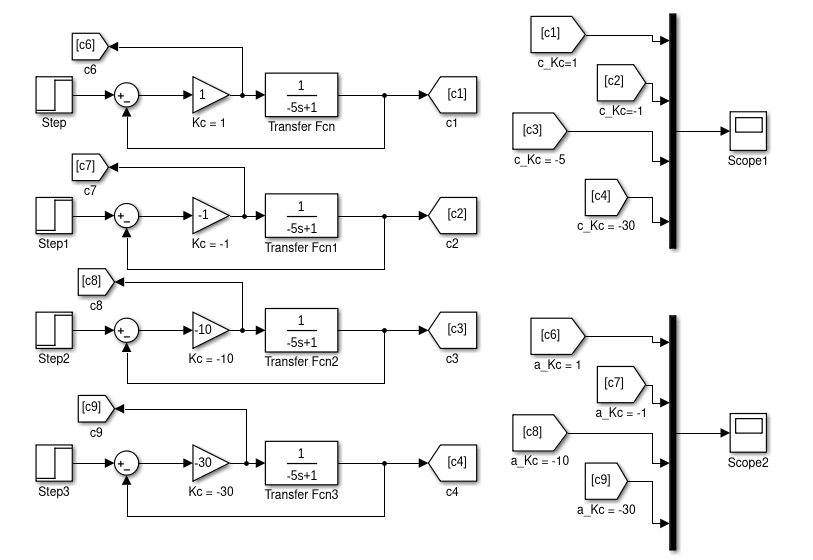
\includegraphics[width = 175mm, scale =0.95]{lab06part10.png}
   \caption{Simulink model of system for proportional control only}
\end{figure}
 \begin{figure}[H]
   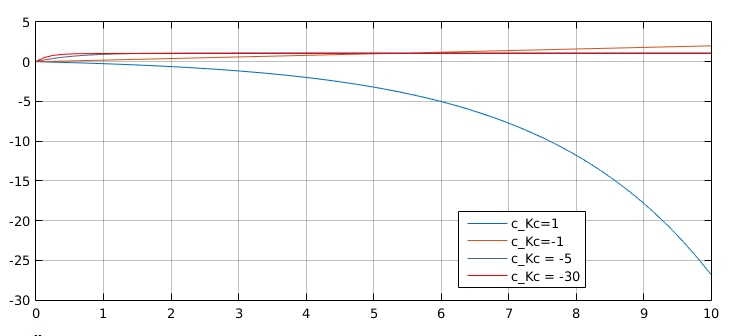
\includegraphics[width = 165mm,  scale = 0.95]{lab06part11.png}
   \caption{step response of systems with different value of $K_c$}
 \end{figure}
 \begin{figure}[H]
   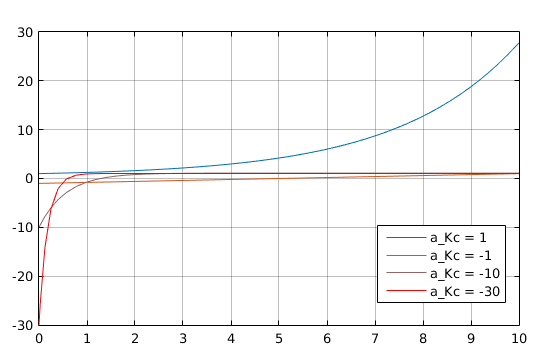
\includegraphics[width = 165mm, height= 90mm, scale = 0.95]{lab06part12.png}
   \caption{controller response of systems with different value of $K_c$}
 \end{figure}
\section{Result : }

\begin{table}[H]
\centering
\resizebox{\textwidth}{!}{%
\begin{tabular}{@{}|l|l|l|l|@{}}
\toprule
\begin{tabular}[c]{@{}l@{}}Proportional Gain\\ Kc\end{tabular} & Output Response & Offset & \begin{tabular}[c]{@{}l@{}}condition of\\ Kp \& Kc\end{tabular} \\ \midrule
1   & Unstable and Unbounded & infinite & Kp Kc \textgreater -1         \\ \midrule
-1  & Unstable and Unbounded & infinite & Kp Kc = -1                    \\ \midrule
-10 & Stable and Bounded     & -0.1     & Kp Kc \textless -1            \\ \midrule
-30 & Stable and Bounded     & -0.03    & Kp Kc \textless{}\textless -1 \\ \bottomrule
\end{tabular}%
}
\caption{step response with varying $K_c$ value}
\label{tab:my-table}
\end{table}





\section{Conclusion : }
\begin{itemize}
  \item step response given to the unstable system gives unbounded output and
    approaches to infinite value
\item from RH's stability criteria we can say that to operate system in stable
  region we need to make $K_c$ < -1, or in more general way it is $K_c$ < 0
\item from varying value $K_c$ to negetive magnitude side we can observe that
  system stabilizes as closed loop right hand side pole effect is dilute huge and
  negetive gain value of $K_c$, in other sense we can get bounded output with
 some amount of offset.  
\end{itemize}

\chapter{Experiment : 08}
\section{Title : Internal Model Control (IMC) based PID controller design for
  $\Romannum{1}^{st}$ Order \& $\Romannum{2}^{nd}$ Order systems}

\section{Apparatus}
MATLAB/Simulink Software

\section{Theory}
\label{sec:lab8_theory}
The most common type of industrial controller is still the PID controller, and 
need of tuning and stabile performance is always desire. so for that we are
using here IMC based controller that can be formulated in the standard feedback
control structure and will result in equivalent PID controller.

\par

PID tuning parameters are tweaked on tranfer function model, but it is not
always clear how the process model effects the tuning decision. In the IMC
formulation the controller $G_c(s)$, is based directly on the ``good'' part of
the process transfer function. \par

The eqauvalent feedback form to IMC
\begin{figure}[ht]
  \centering
  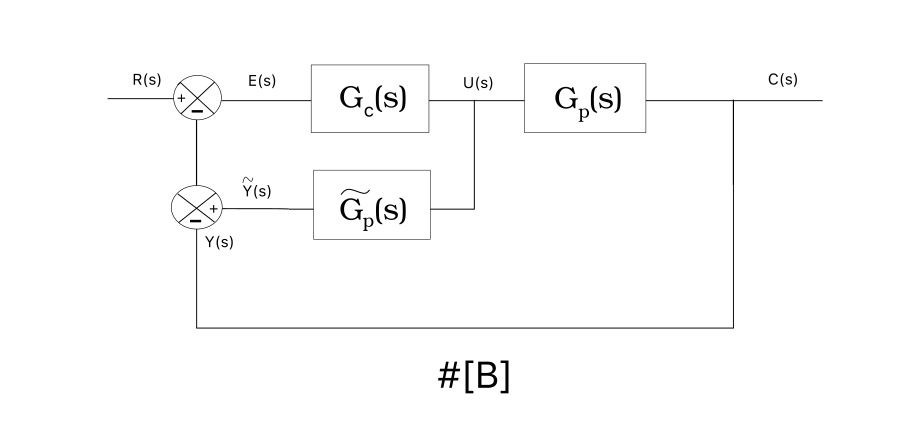
\includegraphics[scale=0.95]{l8p1.png}
  \end{figure}

\end{document}
\message{ !name(lab1.tex) !offset(-637) }
